\begin{flushright} {\tiny {\color{gray} \tt mars\_density\_profile.tex}} \end{flushright}
%~~~~~~~~~~~~~~~~~~~~~~~~~~~~~~~~~~~~~~~~~~~~~~~~~~~~~~~~~~~~~~~~~~~~~~~~~~~~~~~~~~~~~~~~~~~~~~~~~~

\begin{itemize}



%----------------------------------------
\item \fullcite{hard98}

\begin{center}
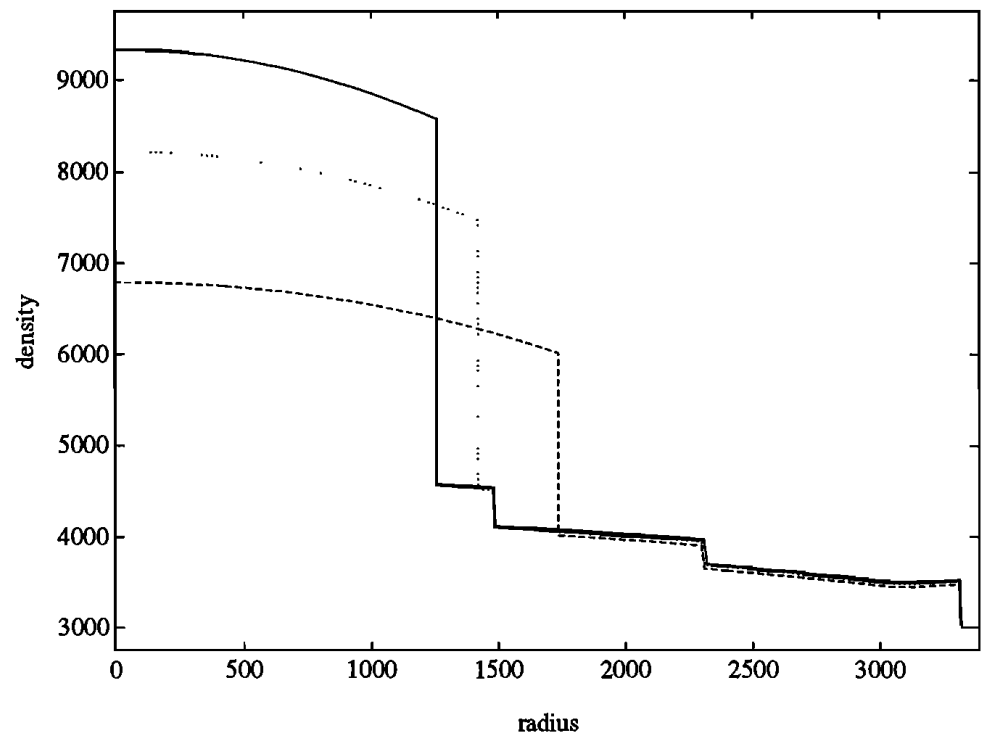
\includegraphics[width=9cm]{images/mars/density/hard98}\\
{\captionfont Possible density structures of Mars' solid(0\%), 
dotted(14\%), and dashed (36.5\%) lines indicate sulphur content of the core.}
\end{center}

%----------------------------------------
\item \fullcite{befe98}

\begin{center}
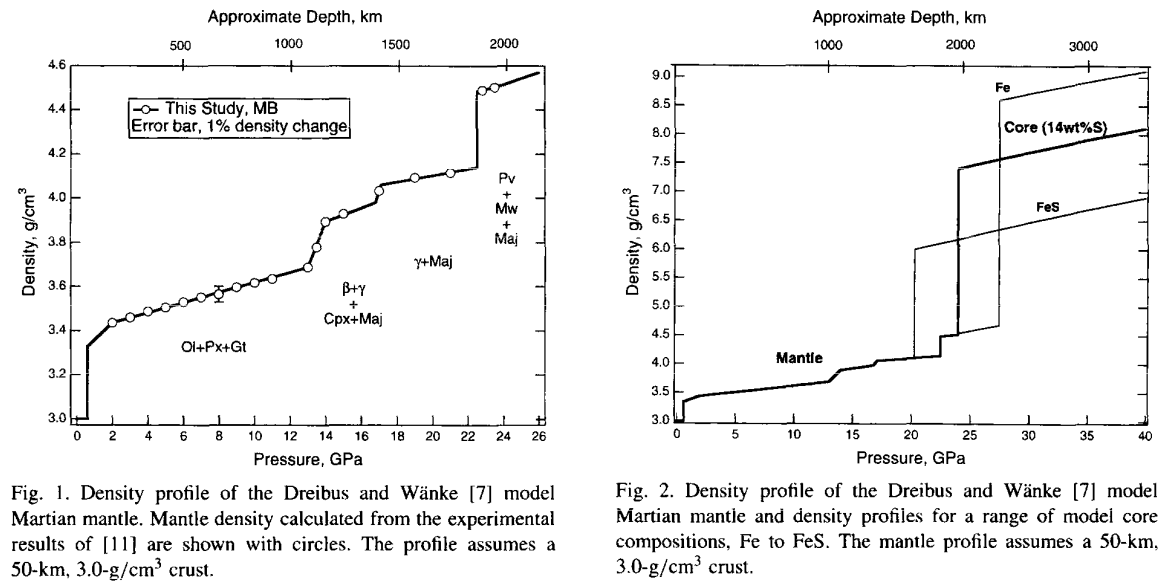
\includegraphics[width=9cm]{images/mars/density/befe98}
\end{center}

%----------------------------------------
\item \fullcite{keta09}

\begin{center}
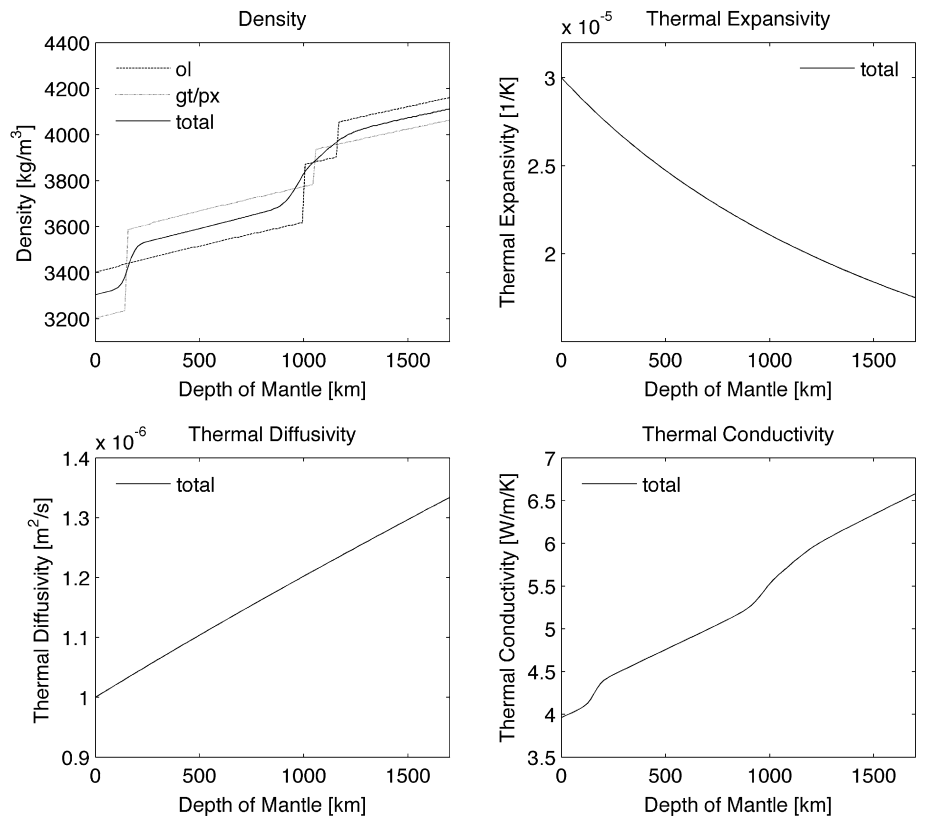
\includegraphics[width=9cm]{images/mars/density/keta09}
\end{center}

%----------------------------------------
\item \fullcite{ruts13}

\begin{center}
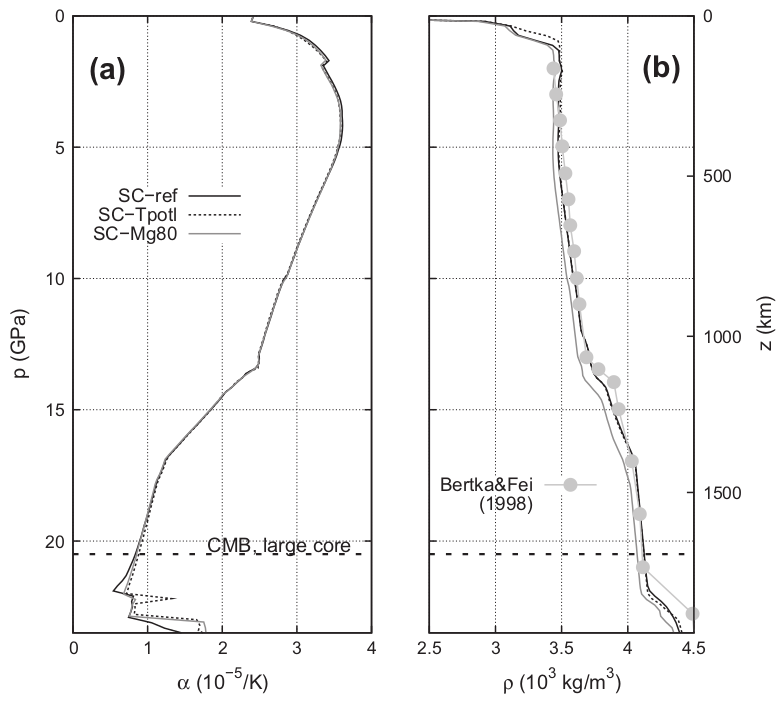
\includegraphics[width=8cm]{images/mars/density/ruts13a}
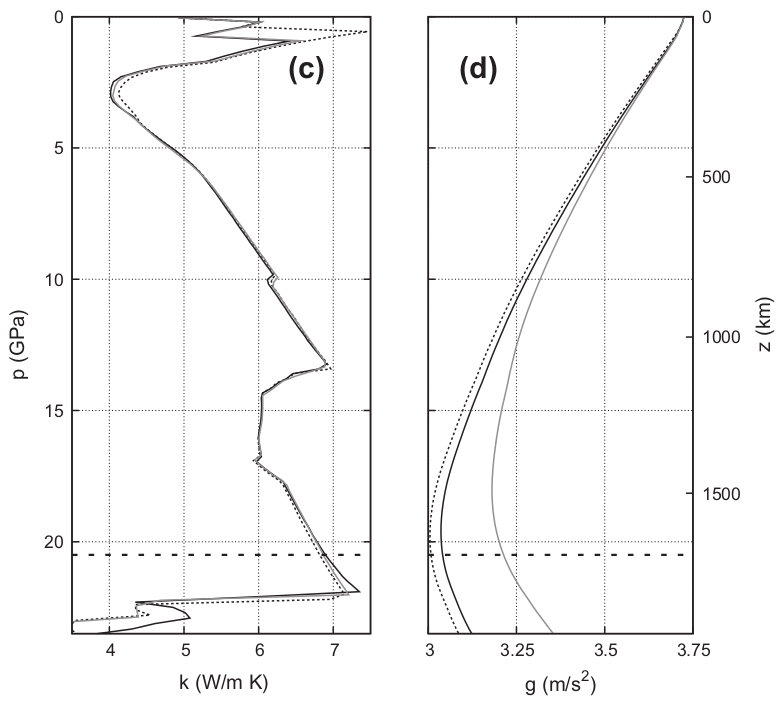
\includegraphics[width=8cm]{images/mars/density/ruts13b}
\end{center}

%----------------------------------------
\item \fullcite{khlr18}

\begin{center}
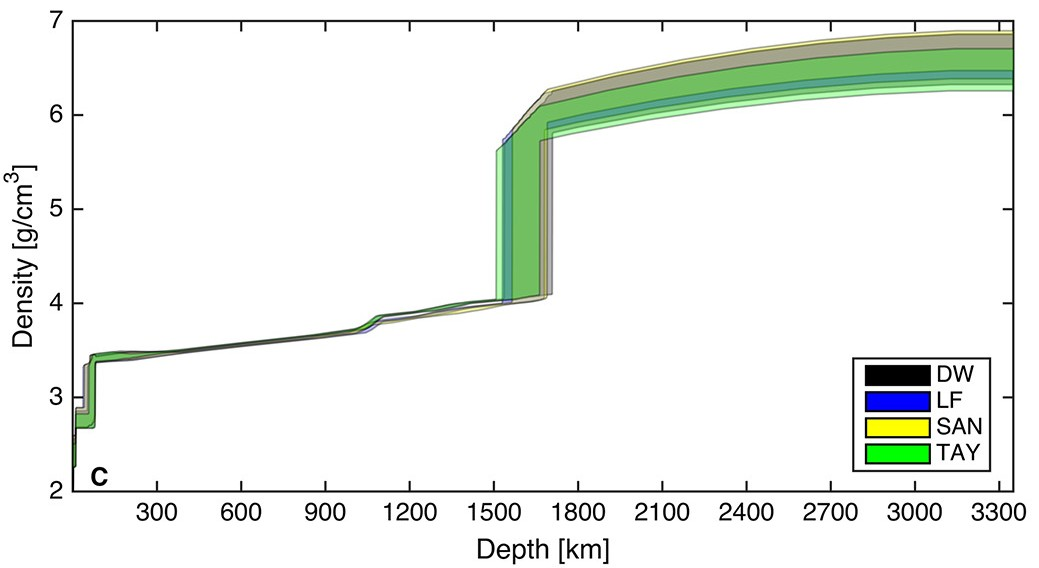
\includegraphics[width=9cm]{images/mars/density/khlr18}
\end{center}

%----------------------------------------
\item \fullcite{smls19}

\begin{center}
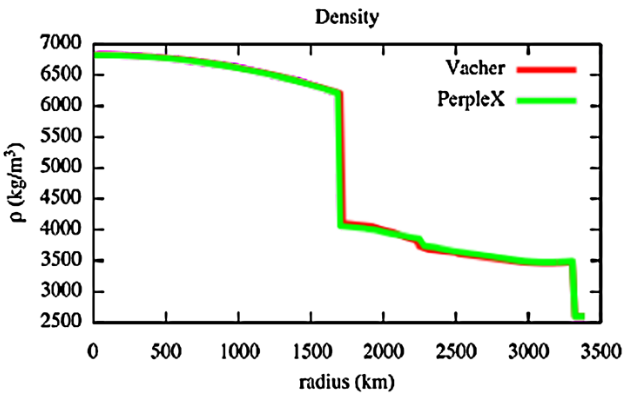
\includegraphics[width=12cm]{images/mars/density/smls19d}
\end{center}

%----------------------------------------
\item \fullcite{brfi20}

\begin{center}
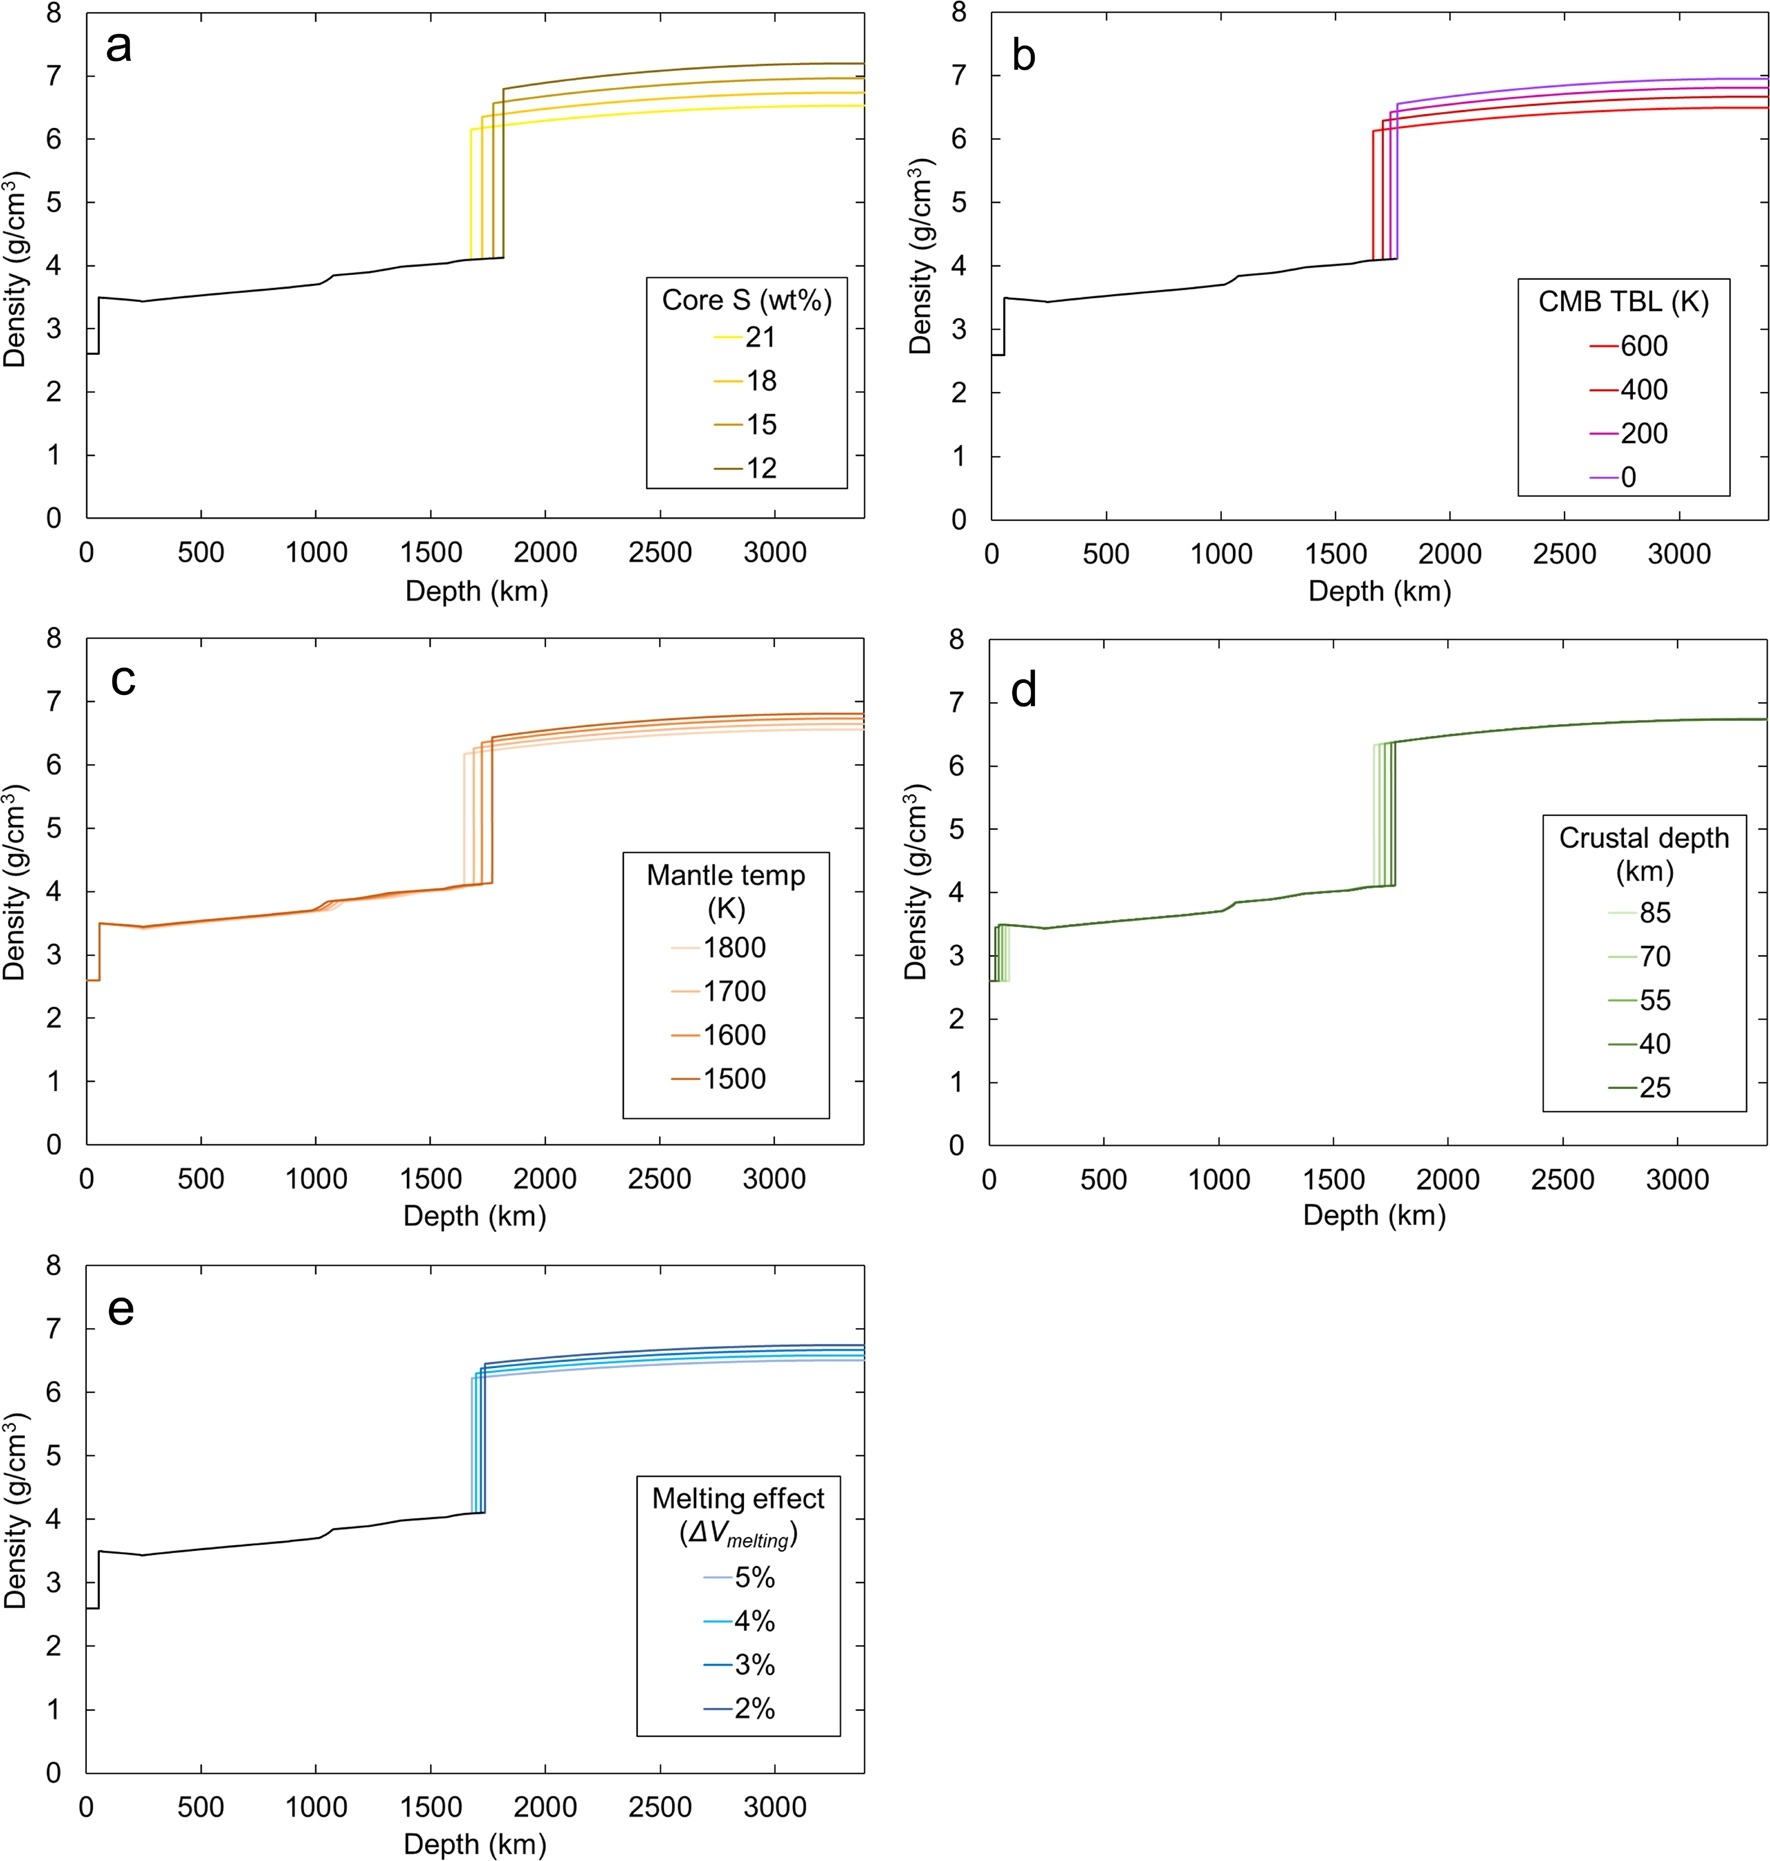
\includegraphics[width=12cm]{images/mars/density/brfi20}
\end{center}

%----------------------------------------
\item \fullcite{plwk22}

\begin{center}
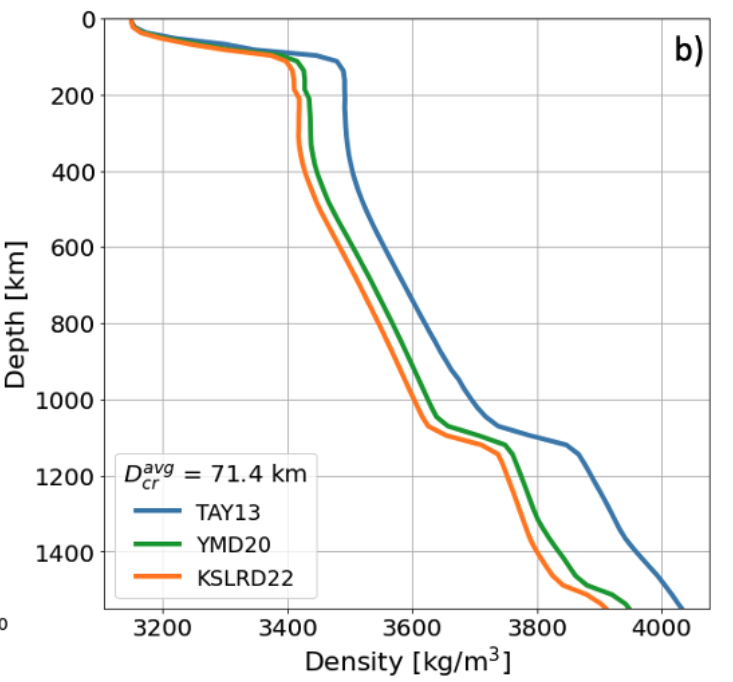
\includegraphics[width=8cm]{images/mars/density/plwk22}
\end{center} 



%----------------------------------------
\item \fullcite{sadr23}

\begin{center}
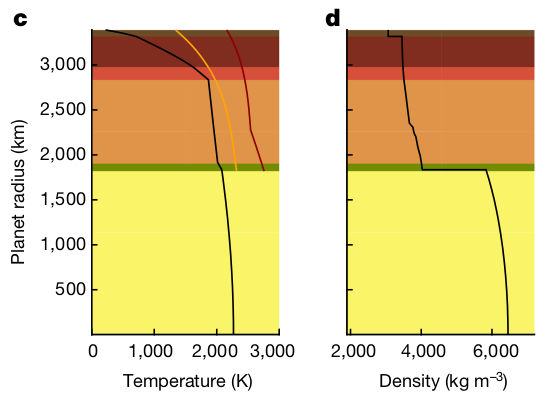
\includegraphics[width=8cm]{images/mars/density/sadr23_a}
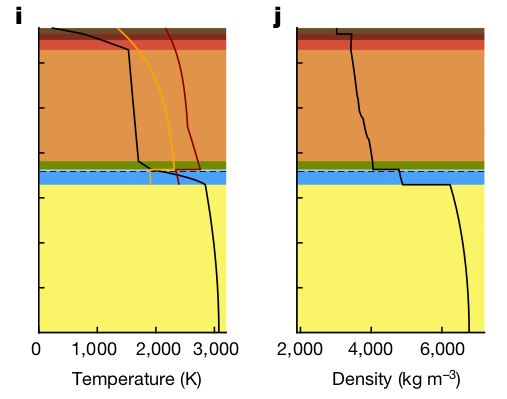
\includegraphics[width=8cm]{images/mars/density/sadr23_b}\\
{\captionfont 
Left: Homogeneous mantle (no basal mantle layer); 
Right: Heterogeneous mantle (with a basal mantle layer)}
\end{center}

\begin{center}
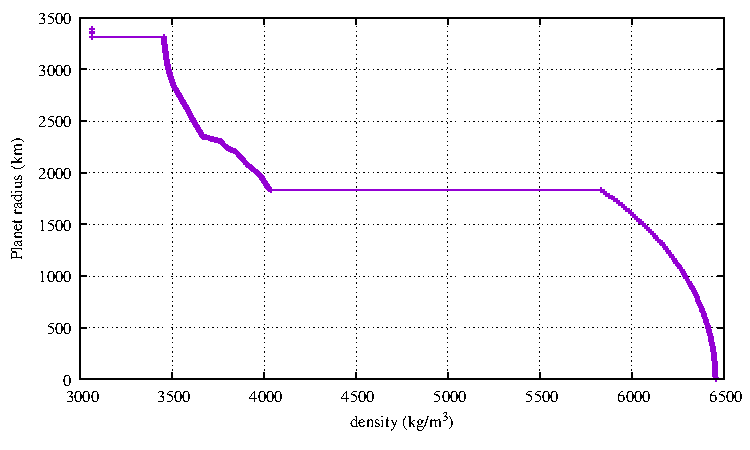
\includegraphics[width=8cm]{images/mars/density/sadr23_fig1d/rho.pdf}
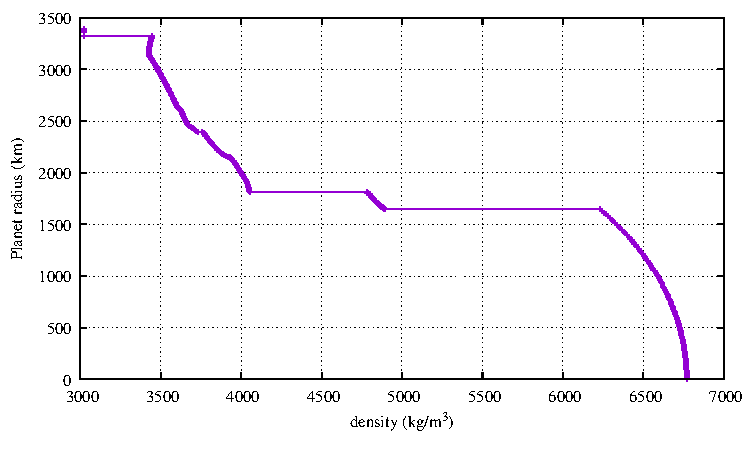
\includegraphics[width=8cm]{images/mars/density/sadr23_fig1j/rho.pdf}\\
{\captionfont Raw data. Left: homogeneous; Right: heterogeneous.}
\end{center} 

%----------------------------------------
\item \fullcite{khhd23}

\begin{center}
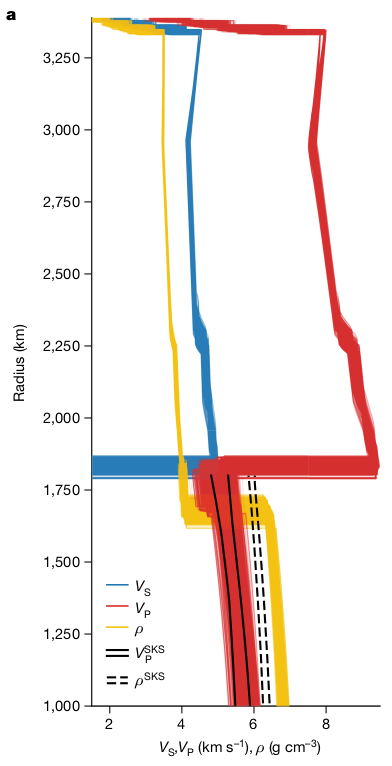
\includegraphics[width=6cm]{images/mars/density/khhd23.png}
\end{center}

There are 1000 profiles in the online data at 
\url{https://dataverse.ipgp.fr/file.xhtml?fileId=3694&version=2.0}.
I have selected about 20 of them to plot:

\begin{center}
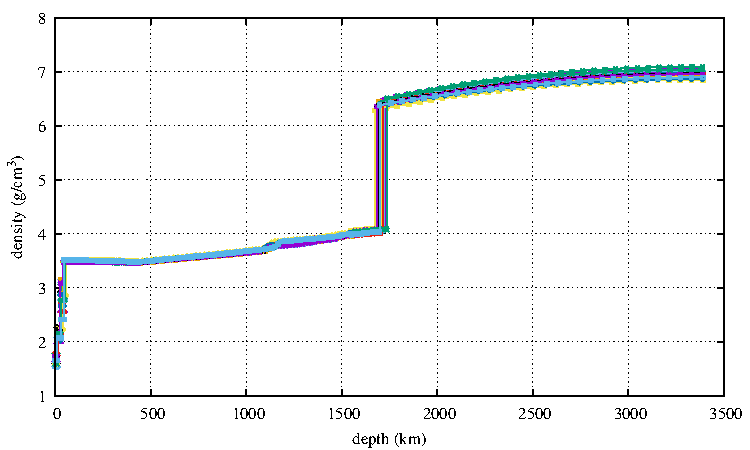
\includegraphics[width=8cm]{images/mars/density/khhd23/rho.pdf}
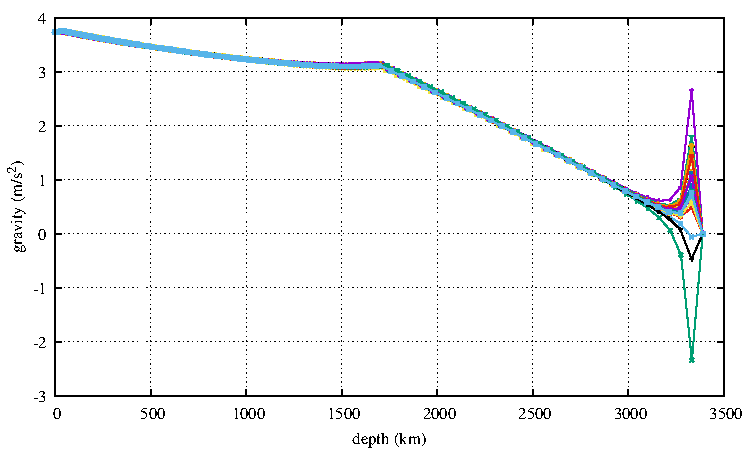
\includegraphics[width=8cm]{images/mars/density/khhd23/g.pdf}
\end{center}

%----------------------------------------
\item \fullcite{gufm24}


\begin{center}
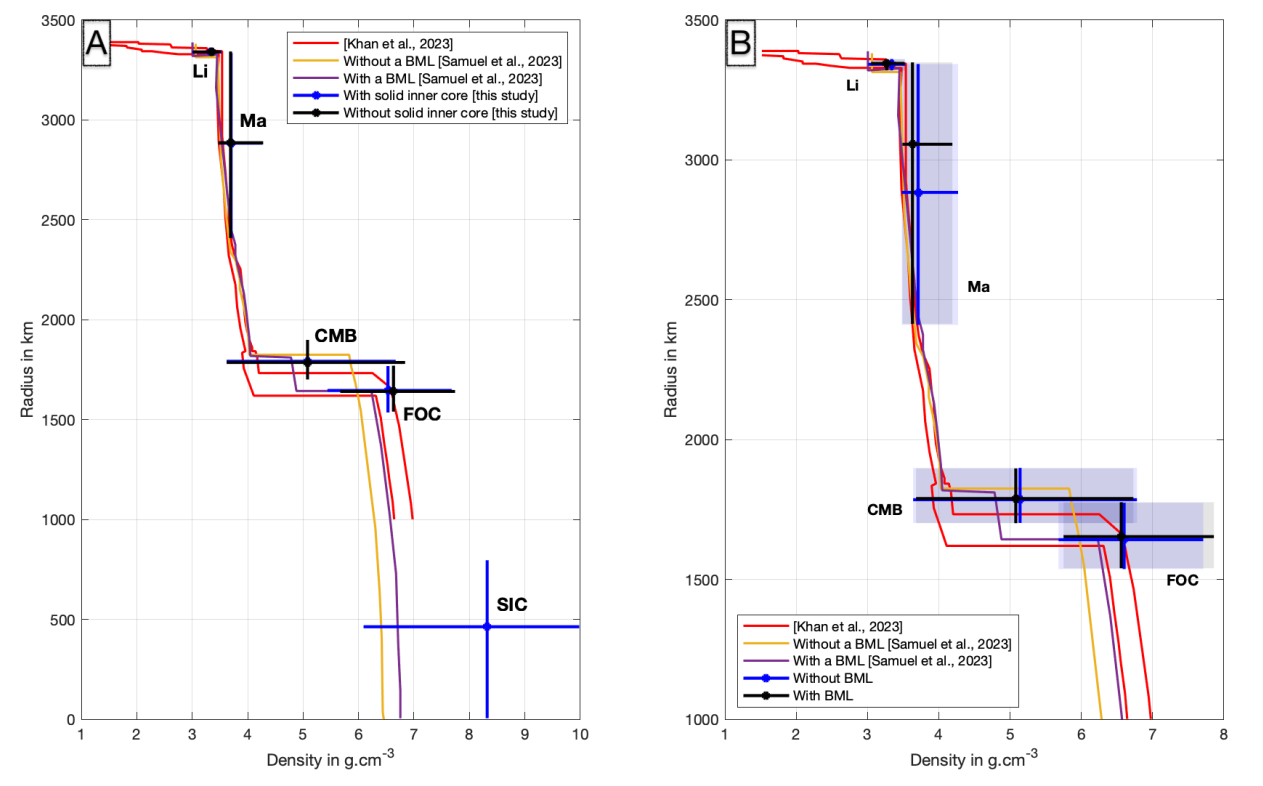
\includegraphics[width=8cm]{images/mars/density/gufm24}
\end{center}

\end{itemize}
